\documentclass[journal]{IEEEtran}
\usepackage[a5paper, margin=10mm, onecolumn]{geometry}
%\usepackage{lmodern} % Ensure lmodern is loaded for pdflatex
\usepackage{tfrupee} % Include tfrupee package

\setlength{\headheight}{1cm} % Set the height of the header box
\setlength{\headsep}{0mm}     % Set the distance between the header box and the top of the text

\usepackage{gvv-book}
\usepackage{gvv}
\usepackage{cite}
\usepackage{amsmath,amssymb,amsfonts,amsthm}
\usepackage{algorithmic}
\usepackage{graphicx}
\usepackage{textcomp}
\usepackage{xcolor}
\usepackage{txfonts}
\usepackage{listings}
\usepackage{enumitem}
\usepackage{mathtools}
\usepackage{gensymb}
\usepackage{comment}
\usepackage[breaklinks=true]{hyperref}
\usepackage{tkz-euclide} 
\usepackage{listings}
% \usepackage{gvv}                                        
\def\inputGnumericTable{}                                 
\usepackage[latin1]{inputenc}                                
\usepackage{color}                                            
\usepackage{array}                                            
\usepackage{longtable}                                       
\usepackage{calc}                                             
\usepackage{multirow}                                         
\usepackage{hhline}                                           
\usepackage{ifthen}                                           
\usepackage{lscape}
\usetikzlibrary{patterns}
\begin{document}
\bibliographystyle{IEEEtran}
\title{2012-XE-'40-52'}
\author{EE24BTECH11009-Mokshith}
{\let\newpage\relax\maketitle}
\renewcommand{\thefigure}{\theenumi}
\renewcommand{\thetable}{\theenumi}
\setlength{\intextsep}{10pt} % Space between text and floats
\numberwithin{equation}{enumi}
\numberwithin{figure}{enumi}
\renewcommand{\thetable}{\theenumi
}
\textbf{Common Data for Questions 19 and 20:}
A boat is propelled in still water at a velocity of $5m/s$ by taking water at the rate of $1m^3/s$ from the aft side and discharging it through the stern using a pump, as shown in the figure below. The velocity of the discharge jet relative to the boat is $9m/s$. The effect of pressure at the intake and discharge can be neglected. The density of water may be taken as $1000kg/m^3$.
\begin{figure}[H]
\centering
\resizebox{7cm}{!}{%
\begin{circuitikz}
\tikzstyle{every node}=[font=\LARGE]
\draw [ line width=1.5pt](-0.5,8.5) to[short] (2.25,11.25);
\node [font=\Huge] at (30.5,8.75) {Discahrge};
\draw [ line width=1.5pt](-0.5,8.5) to[short] (14.5,8.5);
\draw [ line width=1.5pt](2.25,11.25) to[short] (2.25,8.5);
\draw [ line width=1.5pt](2.25,10.75) to[short] (27.5,10.75);
\draw [ line width=1.5pt](27.5,10.75) to[short] (27.5,9.25);
\draw [ line width=1.5pt ] (16.25,7.5) circle (2cm);
\draw [line width=1.5pt, short] (27.5,9.25) -- (17.25,9.25);
\draw [line width=1.5pt, short] (14.5,6.5) -- (-0.5,6.5);
\draw [line width=1.5pt, short] (-0.5,6.5) -- (2,4.25);
\draw [line width=1.5pt, short] (2,4.25) -- (2.25,4);
\draw [line width=1.5pt, short] (2.25,4) -- (2.25,6.5);
\draw [line width=1.5pt, short] (2.25,4.25) -- (27.5,4.25);
\draw [line width=1.5pt, short] (27.5,4.25) -- (27.5,6);
\draw [line width=1.5pt, short] (17.75,6) -- (27.5,6);
\draw [line width=2pt, ->, >=Stealth] (16.25,3.25) -- (16.25,6.5);
\draw [line width=2pt, ->, >=Stealth] (7.25,13) -- (3.25,13);
\draw [line width=2pt, ->, >=Stealth] (26.75,7.5) -- (32.25,7.5);
\node [font=\Huge] at (0.25,3.75) {Aft};
\node [font=\Huge] at (16.25,2.5) {Pump};
\node [font=\Huge] at (28.5,3.25) {Stern};
\node [font=\Huge] at (13.5,13) {Direction of motion of the boat};
\end{circuitikz}
}%
\label{fig:my_label}
\end{figure}
\begin{enumerate}[start=19]
\item The power $\brak{\text{in} kW}$ required to propel the boat is
\begin{enumerate}
    \item 10
    \item 20
    \item 50
    \item 90
\end{enumerate}
\item The total kinetic energy imparted to the water per second $\brak{\text{in} kW}$ by the pump is
\begin{enumerate}
    \item 10
    \item 25
    \item 28
    \item 81
\end{enumerate}
\textbf{Linked Answer Questions}\\
\textbf{Statement for Linked Answer Questions :}
The hydrodynamic boundary layer over a flat plate is shown in the figure below. The velocity in the $x$-direction is approximated as $u = a + by + cy^2$, where $a$, $b$ and $c$ are constants. $U$ is the free stream velocity and $\delta$ is the boundary-layer thickness at any point $x$ on the plate.
\begin{tikzpicture}[scale=1.2, thick]
    % Coordinate system arrows
    \draw[->] (-0.5,0) -- (8,0) node[right] {$x$};
    \draw[->] (0,-0.2) -- (0,2) node[above] {$y$};
    
    % Flat plate with hatching - increased pattern thickness
    \draw[pattern=north west lines, pattern color=black, line width=1.2pt] (0.15,-0.15) -- (8,-0.15);
    \draw[pattern=north west lines, pattern color=black, line width=1.2pt] (0,0) -- (0.15,-0.15);
    % Boundary layer curve - extra thick
    \draw[line width=1.5pt] plot[domain=0:8, smooth] (\x,{0.5*\x^0.5});
    
    % Incoming flow arrows (U) - thicker arrows
    \foreach \y in {0.25,0.75,1.25,1.75}
    {
        \draw[->, line width=1.2pt] (-1.5,\y) -- (-0.5,\y);
    }
    \node[left] at (-1,2) {$U$};
    % Delta(x) height indicator - thicker arrow
    \draw[<->, line width=1.2pt] (6,0) -- (6,1.22474487) node[midway,right] {$\delta(x)$};
\end{tikzpicture}
\item The dimensionless velocity profile is
\begin{enumerate}
    \item $\frac{u}{U} = 2\brak{\frac{y}{\delta}}-\brak{\frac{y}{\delta}}^2$       
    \item $\frac{u}{U} = 2\brak{\frac{y}{\delta}}+\brak{\frac{y}{\delta}}^2$        
    \item $\frac{u}{U} = 1.5\brak{\frac{y}{\delta}}-0.5\brak{\frac{y}{\delta}}^2$        
    \item $\frac{u}{U} = 1.5\brak{\frac{y}{\delta}}+0.5\brak{\frac{y}{\delta}}^2$
\end{enumerate}
\item The displacement thickness $\brak{\text{in} mm}$ when $\delta = 6 mm$, is
\begin{enumerate}
    \item $2.25$
    \item $2$
    \item $-2$
    \item $-2.25$
\end{enumerate}
\end{enumerate}
\section*{C : MATERIALS SCIENCE}
\begin{enumerate}[start=1]
\item Which of the following is NOT a Bravais lattice?
\begin{enumerate}
    \item Simple tetragonal
    \item Body centred tetragonal
    \item Base centred orthorhombic
    \item Face centred tetragonal
\end{enumerate}
\item A Schottky defect in an ionic crystal is a stochiometric defect of
\begin{enumerate}
    \item Cation vacancy
    \item Anion vacancy
    \item Cation and anion vacancy
    \item Cation and anion interstitial
\end{enumerate}
\item Which of the following techniques is NOT used to grow single crystals of semiconductors?
    \begin{enumerate}
    \item Calendering \item Czochralski \item Float zone \item Bridgman
\end{enumerate}
\item Which of the following signals is produced due to the elastic scattering of electrons by a material?
\begin{enumerate}
    \item Secondary electron
    \item Backscattered electron
    \item Auger electron
    \item Photoelectron
\end{enumerate}
\item The best magnetostrictive material is
\begin{enumerate}
    \item $Nd_2Fe_{14}B$ \item $Fe_3O_4$ \item $Cu_2MnAl$ \item $ZnFe_2O_4$
\end{enumerate}
\item Of the following materials, which is the most suitable for an LED emitting at around $380 nm$?
\begin{enumerate}
    \item Direct bandgap material with a small bandgap
    \item Indirect bandgap material with a large bandgap
    \item Direct bandgap material with a large bandgap
    \item Indirect bandgap material with a small bandgap
\end{enumerate}
\item Which material has the lowest specific heat capacity at room temperature?
\begin{enumerate}
    \item Water \item Mercury \item Copper \item Silver
\end{enumerate}
\item Microstrain can be measured by $X$-ray diffraction using peak
\begin{enumerate}
    \item Area and intensity
    \item Position and area
    \item Broadening and intensity
    \item Position and broadening
\end{enumerate}
\item The Pilling-Bedworth ratio is defined as the ratio of
\begin{enumerate}
    \item Volume of oxide to volume of metal
    \item Weight of oxide to weight of metal
    \item Density of oxide to density of metal
    \item Surface area of oxide to surface area of metal
\end{enumerate}
\end{enumerate}
\end{document}
